\documentclass{article}
\usepackage{algorithm}
\usepackage{algorithmic}
\usepackage{amssymb}
\usepackage{graphicx}
\usepackage[letterpaper,margin=1in]{geometry}
\usepackage{listings}

\title{Final Project: Part 2 \\CME 211}
\author{Gabriel Buchsbaum}

\begin{document}
\lstset{language=C++}
\maketitle

\section{Introduction/Summary}

The goal of this project was to create a program that could solve for the thermal gradient in the wall of a pipe carrying hot fluid and cooled by external jets.  This program reads a file with setup information, and uses that to generate a system of equations represented in matrix form that can be solved to find the temperature at each location in the pipe.  This system of equations is then solved, and temporary and final results are saved to a file.  Finally, a second program was written to plot the temperature results, as well as a line tracking the location of the average temperature.

\section{CG solver implementation}

The CG solver relies on two objects plus two additional files: one containing the CG solver function, and one containing additional functions needed for manipulating vectors and matrices. The first object, the \texttt{SparseMatrix}, uses three vectors to represent a sparse matrix (i.e. one in which most of the data is zero and does not need to be specifically stored).  With the equations represented in matrix form as $Ax=b$, this class stores the matrix $A$ (holding the coefficients in the equations).  This class includes functions to add entries, convert to the CSR form for easier calculations, and multiply the matrix by a vector (a function that effectively enters the matrix information into the already-existing function in \texttt{matvecops.cpp}).

The system of equations is set up by a \texttt{HeatEquation2D} object, which contains a \texttt{SparseMatrix} representing $A$ and the vectors $x$ and $b$. The \texttt{HeatEquation2D} reads data from a file to determine the necessary sizes of the matrices and vectors and the temperatures along the borders, then sets up the \texttt{SparseMatrix} to correctly link every data point.  It then is used to input the equations into the \texttt{CGSolver} function.  Since the \texttt{HeatEquation2D} contains information on the area dimensions and the known temperature data, and has more direct access to the desired file name, the function for saving the solution is part of the \texttt{HeatEquation2D} class.

The \texttt{CGSolver} function takes in the \texttt{SparseMatrix} object and the $b$ and $x$ vectors, and uses them to solve the system of equations.  Since a reference to $x$ is passed directly to the function, it can manipulate $x$ directly despite $x$ being a component of the \texttt{HeatEquation2D} class.  The function also takes in a reference to the \texttt{HeatEquation2D} so that it can save the data.  The \texttt{CGSolver} uses the multiplication function from \texttt{SparseMatrix}, as well as several functions from \texttt{matvecops.cpp}, to aid in the calculations.

See Algorithm \ref{pseudocode} for the pseudocode of this algorithm.

\begin{algorithm}
  \caption{CG Solver Pseudocode}
  \label{pseudocode}
  \begin{algorithmic}
    \STATE $u_0 \Leftarrow x$
    \STATE $r_0 \Leftarrow b - A u_0$
    \STATE $L2normr_0 \Leftarrow \|r_0\|_2$
    \STATE $p_0 \Leftarrow r_0$
    \STATE $n_{iter} \Leftarrow 0$
    \WHILE{$n_{iter} < n_{iter,max}$}
      \IF{$n_(iter)$ is divisible by 10}
        \STATE Save results
      \ENDIF
      \STATE $n_{iter} \Leftarrow n_{iter} + 1$
      \STATE $\alpha_n \Leftarrow \left(r_n^\intercal r_n \right) \left(p_n^\intercal A p_n \right)$
      \STATE $u_{n+1} \Leftarrow u_n + \alpha_n p_n$
      \STATE $r_{n+1} \Leftarrow r_n - \alpha_n A p_n$
      \STATE $L2normr \Leftarrow \|r_{n+1}\|_2$
      \IF{$\frac{L2normr}{L2normr_0} < \epsilon$}
        \STATE \textbf{break}
      \ENDIF
      \STATE $\beta_n \Leftarrow \frac{r_{n+1}^\intercal r_{n+1}} {r_n^\intercal r_n}$
      \STATE $p_{n+1} \Leftarrow r_{n+1} + \beta_n p_n$
    \ENDWHILE
    \IF{Desired tolerance not achieved}
      \STATE Report error and exit
    \ENDIF
    \STATE $x \Leftarrow u_{n+1}$
    \RETURN $n_{iter}$
  \end{algorithmic}
\end{algorithm}

\section{User guide}

The file \texttt{makefile} can perform can compile the program easily, just by using the \texttt{make} command.

\begin{verbatim}
$ make
g++ -c -o main.o main.cpp -std=c++11 -O3 -Wall -Wextra -Wconversion -Wpedantic
g++ -c -o CGSolver.o CGSolver.cpp -std=c++11 -O3 -Wall -Wextra -Wconversion -Wpedantic
g++ -c -o COO2CSR.o COO2CSR.cpp -std=c++11 -O3 -Wall -Wextra -Wconversion -Wpedantic
g++ -c -o matvecops.o matvecops.cpp -std=c++11 -O3 -Wall -Wextra -Wconversion -Wpedantic
g++ -c -o heat.o heat.cpp -std=c++11 -O3 -Wall -Wextra -Wconversion -Wpedantic
g++ -c -o sparse.o sparse.cpp -std=c++11 -O3 -Wall -Wextra -Wconversion -Wpedantic
g++ -o main main.o CGSolver.o COO2CSR.o matvecops.o heat.o sparse.o
\end{verbatim}

The \texttt{makefile} can also remove the object and editor files, as well as \texttt{main}:

\begin{verbatim}
$ make clean
rm -f *.o *~ main
\end{verbatim}

To use the program, it must be provided with a correctly-formatted input file. The first row of the file contains the length and width of the zone being solved for, then the separation of points in the solution.  The second row contains the temperature of the hot boundary and the temperature of the cold jet.  For example:

\begin{verbatim}
$ cat input2.txt
1.0 0.3 0.005
30 120
\end{verbatim}

The user needs to provide \texttt{main} with this file, as well as a prefix to use for the solution files:

\begin{verbatim}
$ ./main input2.txt solution
SUCCESS: CG solver converged in 157 iterations.
$ ls solution*.txt
solution000.txt  solution050.txt  solution100.txt  solution150.txt
solution010.txt  solution060.txt  solution110.txt  solution157.txt
solution020.txt  solution070.txt  solution120.txt
solution030.txt  solution080.txt  solution130.txt
solution040.txt  solution090.txt  solution140.txt
\end{verbatim}

The user can then run the post processing script by giving it the original input file and the final solution file\footnote{This can also work on intermediate solutions, although the results will obviously not be correct}:

\begin{verbatim}
$ python3 postprocess.py input2.txt solution157.txt
Input file processed: input2.txt
Mean Temperature: 81.80566
\end{verbatim}

\texttt{postprocess.py} will also save the plot as an image with the same name as the solution file, albeit with the \texttt{.png} extension, i.e. \texttt{solution157.png}.

To run the bonus animation, the same input as \texttt{postprocess.py} is used.  While every intermediate solution file is used, the program can determine these intermediate file names from the last file name.

\begin{verbatim}
$ python3 bonus.py input2.txt solution157.txt
Input file animated: input2.txt
\end{verbatim}

\texttt{bonus.py} saves the animation using a similar convention, i.e. \texttt{solution157.mp4}.  It does require the \texttt{ffmpeg} writer to save the file.  An example has been uploaded, in case the code does not function in the environment being used.

\section{Images}

\begin{figure}[htb]
  \begin{center}
    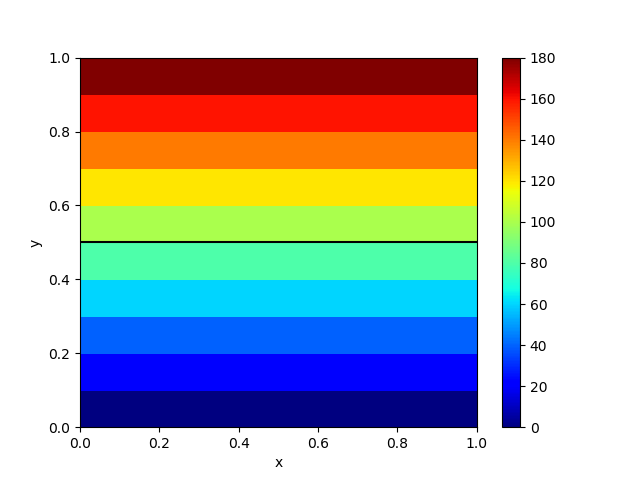
\includegraphics[width=0.75\linewidth]{solution0009.png}
    \caption{Post processing results for \texttt{input0.txt}}
    \label{fig:input0}
  \end{center}
\end{figure}

\begin{figure}[H]
  \begin{center}
    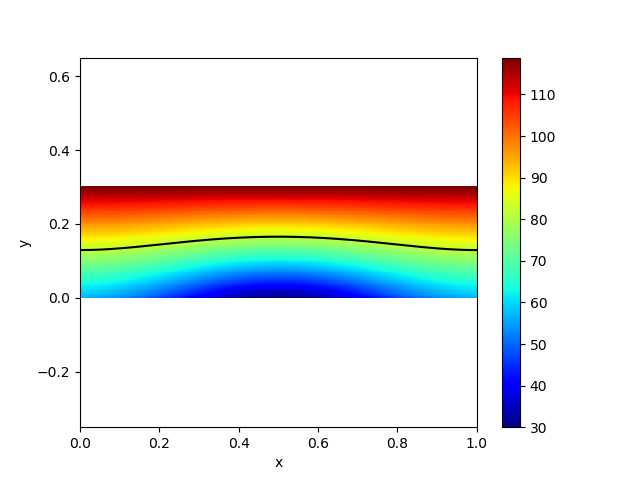
\includegraphics[width=0.75\linewidth]{solution157.png}
    \caption{Post processing results for \texttt{input2.txt}}
    \label{fig:input2}
  \end{center}
\end{figure}

\nocite{*}
\bibliographystyle{unsrt}
\bibliography{references}

\end{document}
